\documentclass[12pt,a4paper]{report}

%Set language
\usepackage[english]{babel}
\usepackage{enumerate}

% To import and adjust images
\usepackage{graphicx}
\usepackage[export]{adjustbox}
\usepackage[center]{caption}
\usepackage{subcaption}
\usepackage{float}
\usepackage{tabularx}

% To use monospaced font
\usepackage{courier}

% To build a clickable Toc
\usepackage{color} %May be necessary if you want to color links
\usepackage{hyperref}
\hypersetup{
    colorlinks=true, %set true if you want colored links
    linktoc=all,     %set to all if you want both sections and subsections linked
    linkcolor=black,  %choose some color if you want links to stand out
    urlcolor = black
}


%To load PoLitecnico's logo
\usepackage{titling}

% Command to hide subsections in the Toc
\setcounter{tocdepth}{1}

% I don't like dots in the Toc
\usepackage{tocloft}
\renewcommand{\cftdot}{}

%To improve the tables
\usepackage[table]{xcolor}

%To break line inside tables
%\usepackage[utf8]{inputenc}
%\usepackage{fourier} 
%\usepackage{array}
\usepackage{makecell}
%\renewcommand\theadalign{bc}
%\renewcommand\theadfont{\bfseries}
\renewcommand\theadgape{\Gape[4pt]}

% Path relative to the .tex file containing the \includegraphics command
\graphicspath{ {./images/} }

% To change the ToC title
\addto\captionsenglish{ \renewcommand {\contentsname} {Table of
contents}}

%logo
\pretitle{
	 \begin{center}
	 \LARGE
	 
\includegraphics[width = 0.6\textwidth]{logo}\\[\bigskipamount]
}
\posttitle{\end{center}}

% Here we go
\title{Artificial Neural Networks and Deep Learning \\ Homework 2 - Image Segmentation}
\author{Frantuma Elia - 10567359 - 945729, \\
		Fucci Tiziano - 10524029 - 946638}
\date{A.Y. 2020/2021}

\begin{document}
	\maketitle
	%Index
	\tableofcontents
	\chapter{Introduction}
		\section{Description of the task}
			The homework consists in an image segmentation problem on the proposed dataset. In particular, it is required to segment RGB images to distinguish between crop, weeds, and background, as done in the following example.

\begin{figure}[H]
\renewcommand*\thesubfigure{\arabic{subfigure}} 
\centering
\begin{subfigure}{.45\textwidth}
  \centering
  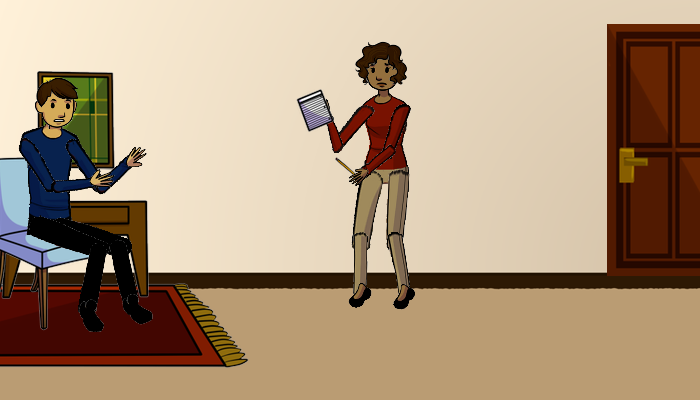
\includegraphics[width=1\linewidth]{image0}
  \caption{dataset image}
  \label{fig:sub1}
\end{subfigure}
\begin{subfigure}{.45\textwidth}
  \centering
  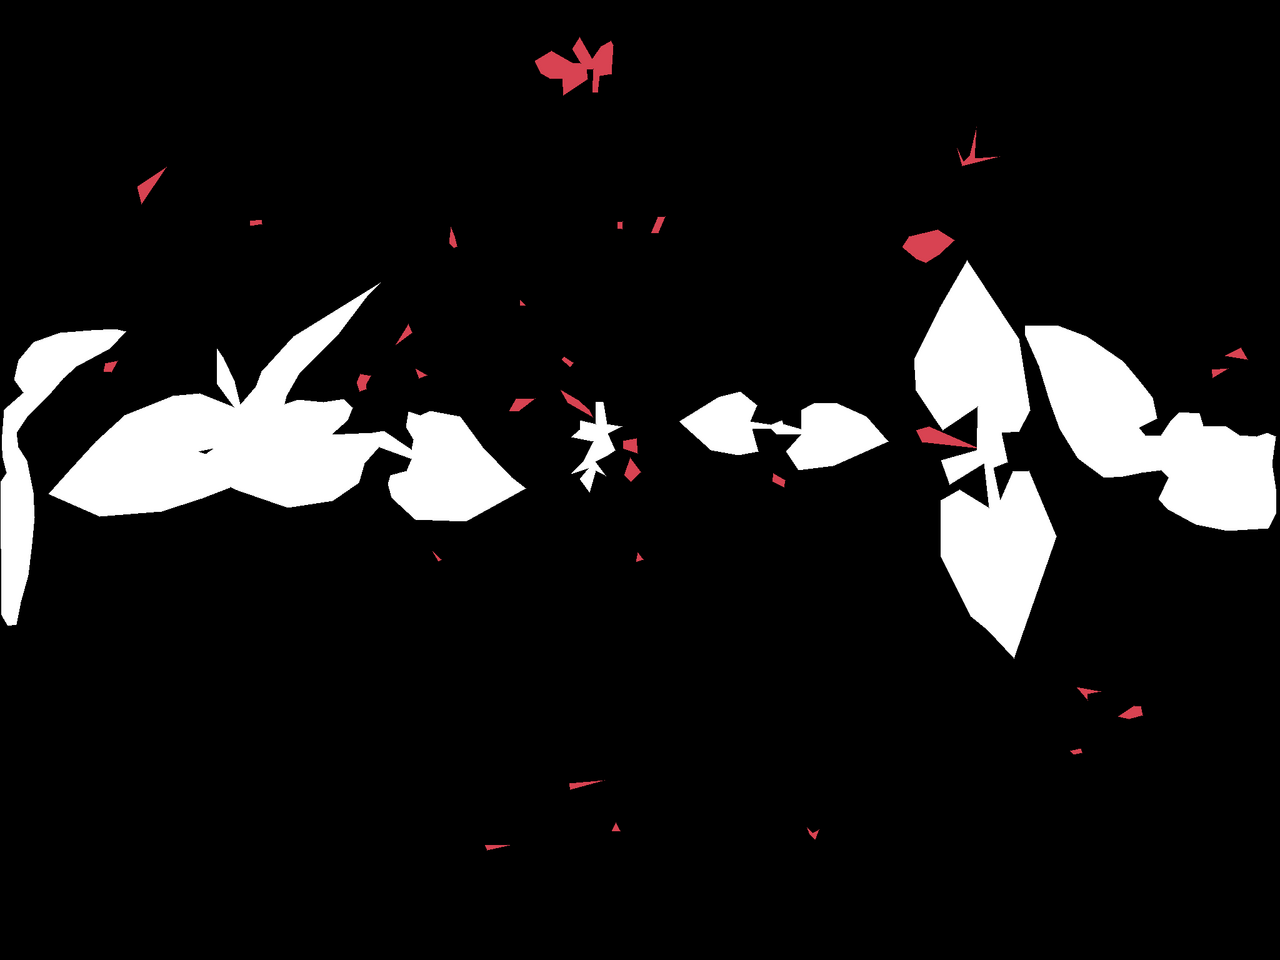
\includegraphics[width=1\linewidth]{image1}
  \caption{segmented image}
  \label{fig:sub2}
\end{subfigure}
\end{figure}

The competition is public and  organized by the ACRE (Agri-food Competition for Robot Evaluation).

	\section{Dataset}
The dataset is composed of images captured by different sensors in different moments and are about two kinds of crops: haricot and maize. Data comes from the 2019 ROSE Challenge where four teams have competed with agricultural robots. Each team has collected images of the same two crops, but in different moments and with different sensors (RGB cameras).

Images in the dataset are divided into different folders based on the team that acquired the image, i.e., Bipbip, Pead, Roseau, Weedelec. For each team, we have two different sub-folders named as the type of crop present in the images, i.e., Haricot and Mais. Finally, for each crop, the captured RGB images (in the Images folder) and the corresponding ground-truth segmentations (in the Masks folder) are provided.
	
We decided to apply for maize from the Bipbip dataset.
	\subsection{Images}
Teams' images share most of the properties but differ from image size and file format. The common properties are:
\begin{itemize}

\item{color space: RGB;}
\item{classes:}
\begin{itemize}
\item{crop;}
\item{weed;}
\item{background;}
\end{itemize}
\item{number of Training images (per team per crop): 90;}
\item{number of Test\_Dev images (per team per crop): 15;}
\item{number of Test images (per team per crop): 20.}
\end{itemize}
	\subsection{Masks}
Masks folders contain the ground-truth segmentation for each corresponding (having the same name) image in the Images folder. They have the same exact properties of the Images set apart from the fact that they all have the same file format: PNG.

In each mask, classes are represented by different colors. The dictionary which allows assigning a label to each corresponding color is provided in the starting\_kit, as well as the example script in which we show how to transform RGB masks into target masks. In the following, the provided dictionary ('RGBtoTarget.txt' in the starting kit):
			\begin{itemize}
				\item RGB: 0 0 0 - Target 0 (background);
				\item RGB: 254 124 18 - Target 0 (background);
				\item RGB: 255 255 255 - Target 1 (crop);
				\item RGB: 216 67 82 - Target 2 (weed).
			\end{itemize}

	\subsection{Data augmentation}
We have performed data augmentation in order to increase the dataset dimension. Some of the parameters used to perform the transformations are: rotation, zoom, horizontal/vertical shift and flip.

	\subsection{Tiling}
During the training, we have experienced many issues with the RAM and VRAM. This happened both with Colab Pro and local tests. We decided not to downsize the dataset images, since the quality loss would have been too much, so we performed image tiling. In the final version, we splitted the original images into 8 tiles per image.

	\section{Validation set}

No automatic validation set is provided. This means that a subset of the training set must be used to perform validation.

In our case, we parametrized the number of training images to be moved into the validation set, with a 10\% probability.


	\section{Test set}
Test\_Dev images are provided without any ground-truth mask. Participants are required to provide the segmentations for the Test\_Dev images by submitting the solution with the correct submission format. 
	\section{Evaluation}
Submissions are evaluated on the mean Intersection over Union (IoU) obtained on the two classes, crop and weed. IoU is computed for each target class (crop and weed) separately, by considering prediction and ground truth as binary masks. Then, the final IoU is computed by averaging the two.

	%end of first chapter

	\chapter{Neural network architecture}		
For all the networks, we have modified the function \texttt{read\_mask\_example}. The modified function can be found into the \texttt{starting\_kit} folder. The notebook expects that folder to be in \texttt{\textbackslash content\textbackslash drive\textbackslash MyDrive}.
		\section{U-Net}
Our first try was with U-Net, but the results turned out to be very poor. In particular, the high number of parameters made the tuning very difficult to perform. The training time was simply too much to experience some progress, since it took up to one hour and a half for one epoch. After some epoch, the result was the one shown below. 
\begin{figure}[H]
	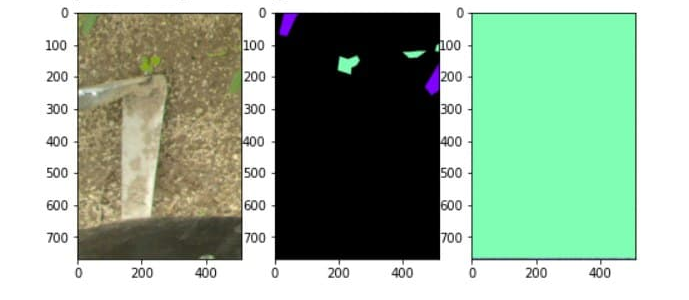
\includegraphics[scale = .75, center]{U_Net}
	\caption{dataset image, target segmentation, actual segmentation}
\end{figure}
	
We tried to change the learning rate, the weights initialization and the loss function, using a weighted one, but the situation remained the same.	
		
		\section{Transfer learning with MobileNetV2}
Then, we tried to use MobileNetV2, as it was suggested by the TensorFlow tutorial. After a while, we noticed that the trained model could not distinguish the maize plants from weeds. The result was a well defined foreground, but with a faded violet, since the two colours were mixed in correspondence of the plant.  This was probably caused by the incompatibility of the weights with non-squared images, as shown by Jupyter in a warning. 
	

\begin{figure}[H]
	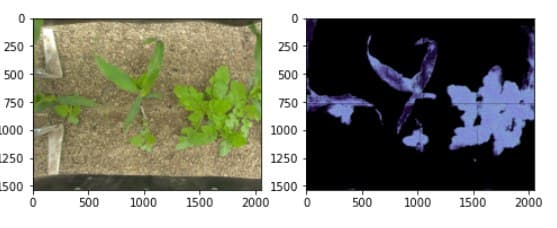
\includegraphics[scale = 1.2, center]{MobileNetV2}
	\caption{image segmentation}
\end{figure}

		\section{U-Net, with VGG as a backbone}
	\subsection{Without skip connections}
This architecture is taken from the notebooks seen during the exercise sessions of the course, adapted to this competition.
After some epochs, the results were similar to the one shown below.

\begin{figure}[H]
	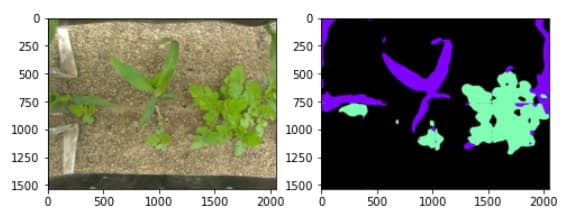
\includegraphics[scale = .75, center]{vgg_upsampling_without}
	\caption{image segmentation}
\end{figure}
	\subsection{With skip connections}
\begin{figure}[H]
	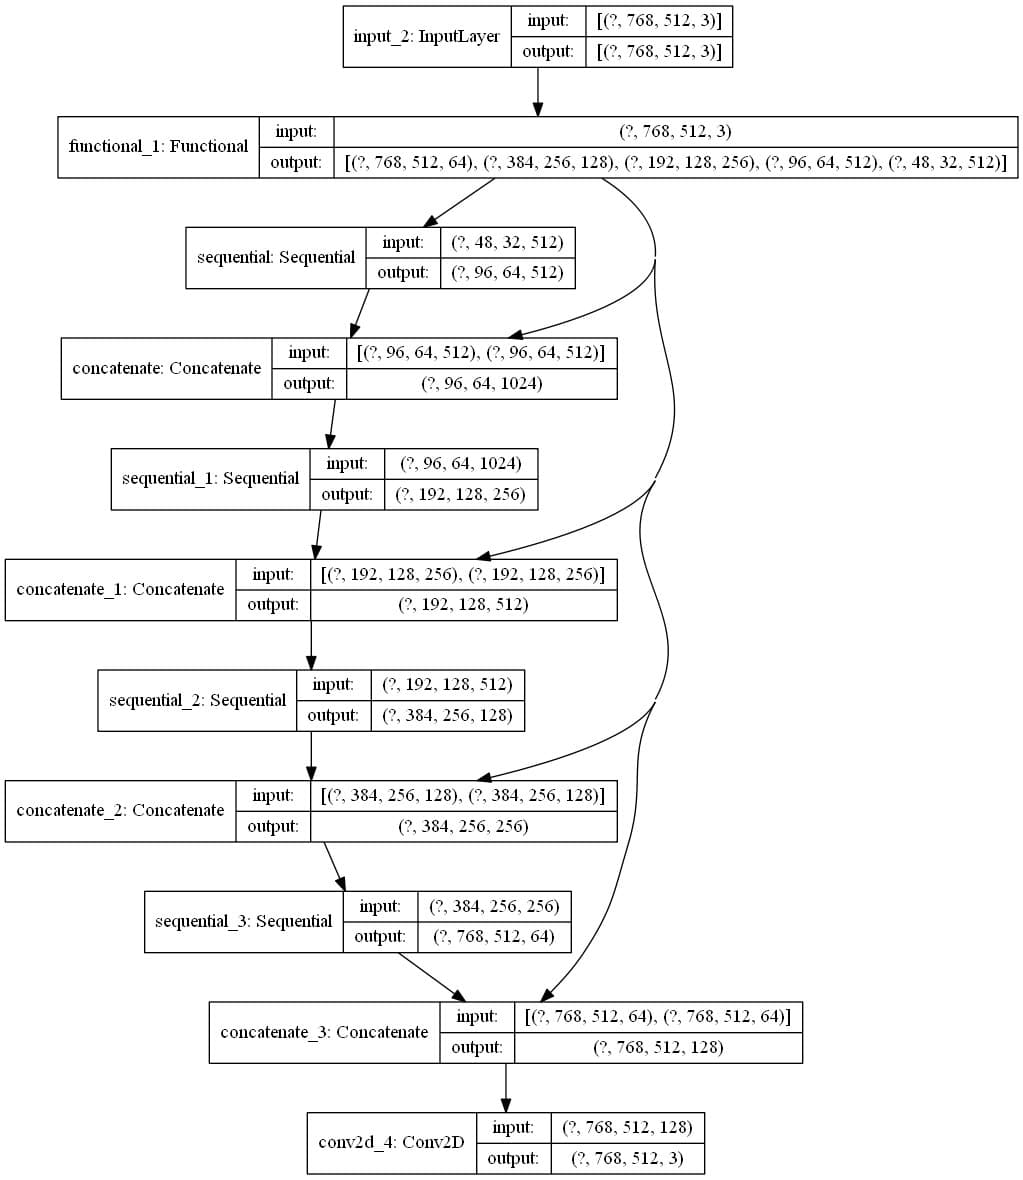
\includegraphics[scale = .45, center]{vgg_model}
	\caption{network obtained with VGG and skipped connections}
\end{figure}
After considering the former architecture, we decided to add skip connections in order to improve the performance of the upsampling layers. This led to a better definition of shapes and leaves and thus to a higher score.
\begin{figure}[H]
	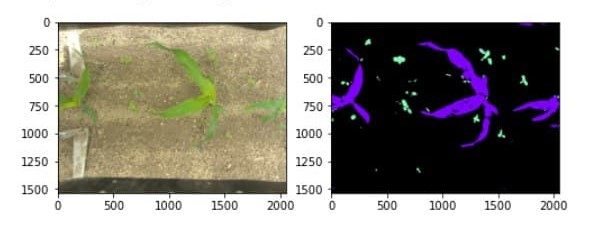
\includegraphics[scale = .75, center]{vgg_upsampling_with}
	\caption{image segmentation}
\end{figure}
\subsection{Score}
	The best score of the network was 0.7207, obtained with the skip connections.
		
	%end of second chapter

\chapter{Main issues}
During this competition we had to face problems that didn't occur in the first one: despite we could solve memory capacity issues by tiling the images, the main problem remained time. The classic network tuning procedure has been hardened by the great training time, up to one hour per epoch (obtained with U-Net). Even with the other network architectures, the training time was so long that it took hours, or days, to understand if the network was properly learning the model. This was the main reason because we used the Maize dataset only.

The tiling procedure took so long (8-10 hours) that we could not make many attempts on how many tiles were better. Furthemore, we had to manually fix the folder structure in the .zip file, since Colab didn't allow us to recreate the original dataset structure.

Other factors that limited our score were the absence of the last softmax layer and the TensorFlow preprocessing of predictions for VGG, that drastically lowered the performance of the network. We managed to correct these two mistakes just in the last days.
	%end of third chapter
	\chapter{References}
		\section{Links}

\begin{itemize}
	\item GitHub repository of the project: \url{https://github.com/tizianofucci/A2NDLSegmentation}
	\item Competition web page: \url{https://competitions.codalab.org/competitions/27176}
\end{itemize}

\end{document}
